\begin{wrapfigure}[0]{r}[-3.5cm]{3cm}
 \vspace{-6cm}
 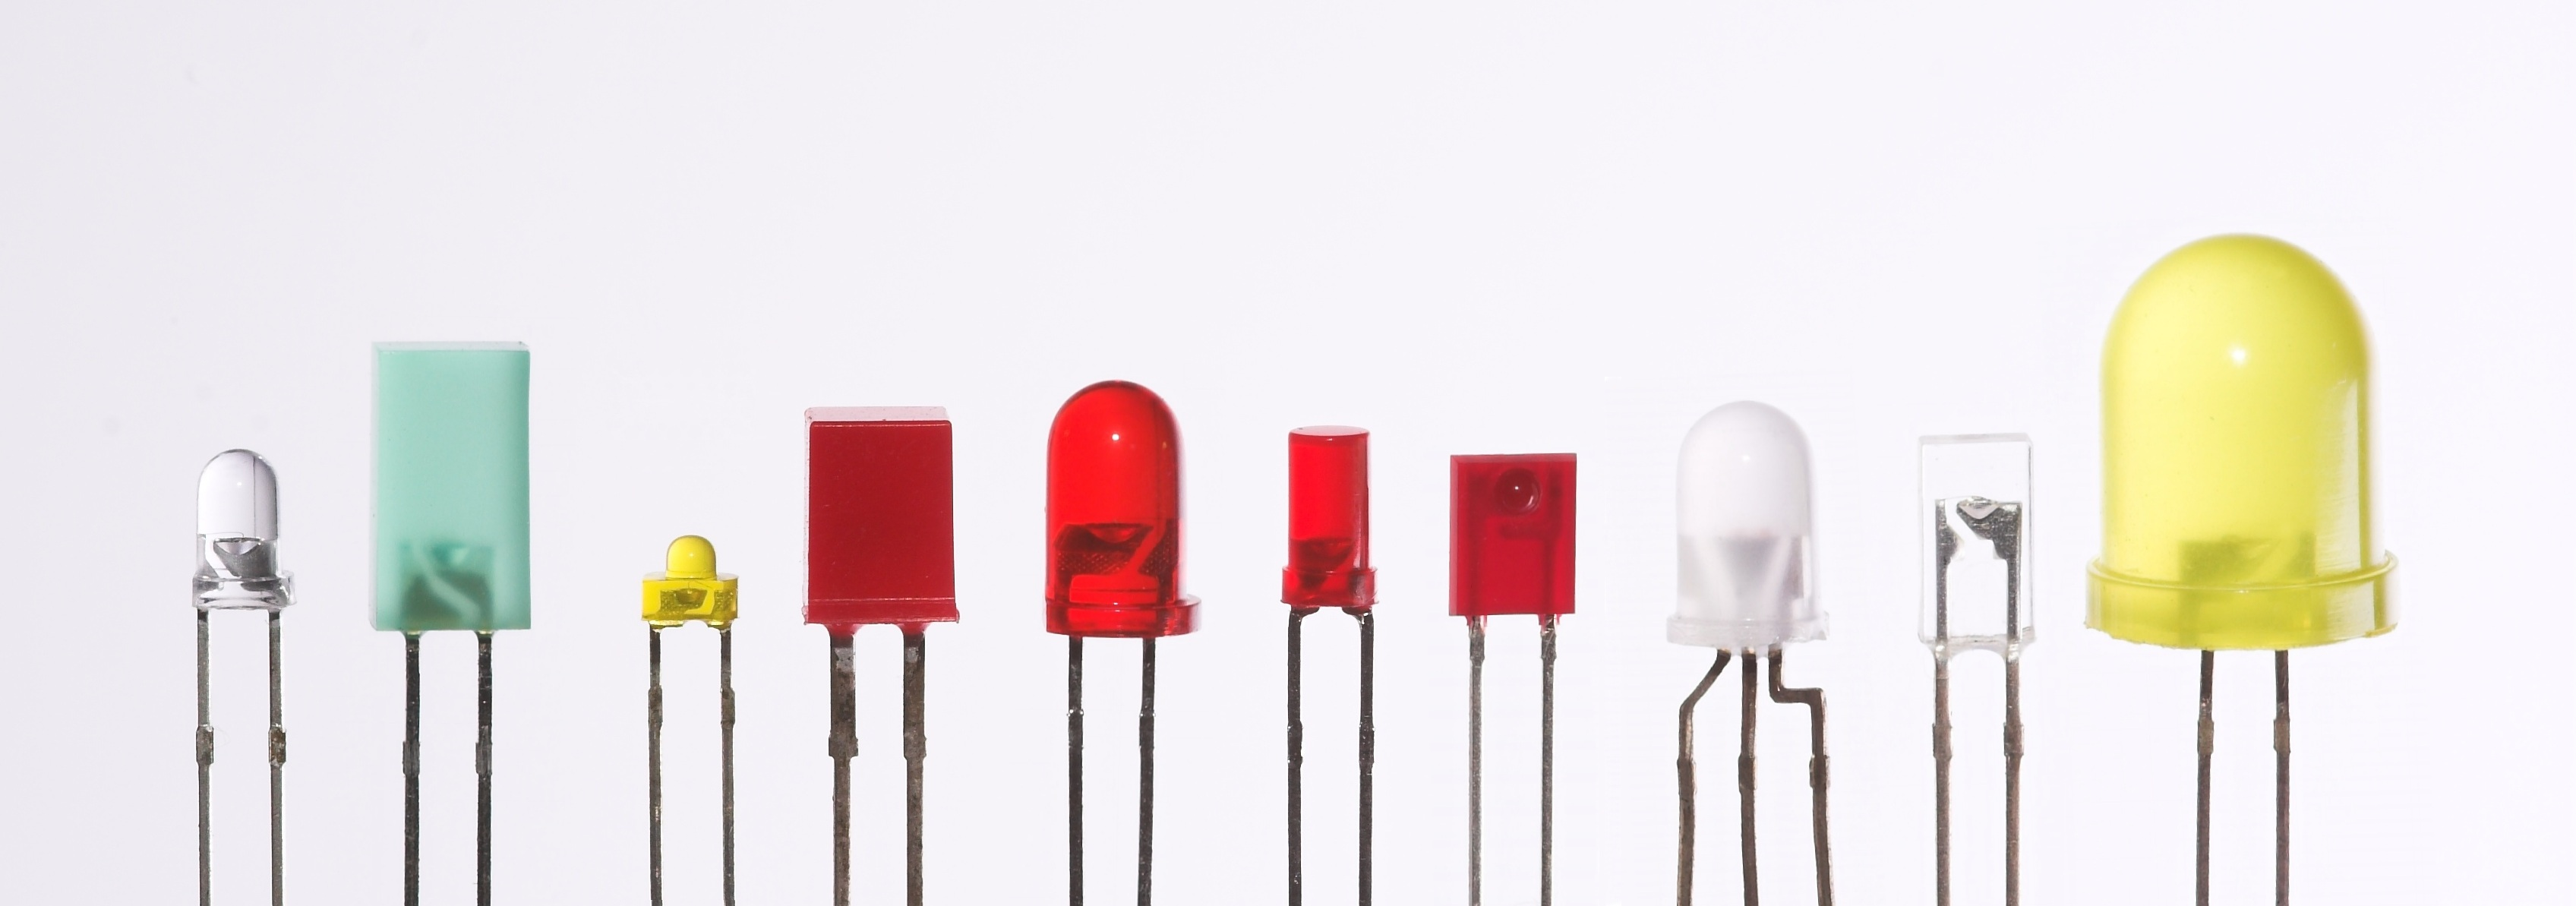
\includegraphics[scale=0.25]{Diode/Bilder/Verschiedene_LEDs.jpg}
 \vspace{-6cm}
\end{wrapfigure}

\section*{Theorie- und Prüfungsfragen} 


\mucho{1}{TB106}s
{Was versteht man unter Halbleitermaterialien?}%Frage
{Einige Stoffe (z.B. Silizium, Germanium) sind in reinem Zustand bei Zimmertemperatur gute Leiter. Durch geringfügige Zusätze von geeigneten anderen Stoffen oder bei hohen Temperaturen nimmt jedoch ihre Leitfähigkeit ab.}%A
{Einige Stoffe (z.B. Silizium, Germanium) sind in reinem Zustand bei Zimmertemperatur gute Isolatoren. Durch geringfügige Zusätze von geeigneten anderen Stoffen oder bei hohen Temperaturen werden sie jedoch zu Leitern.}%B
{Einige Stoffe wie z.B. Indium oder Magnesium sind in reinem Zustand gute Isolatoren. Durch geringfügige Zusätze von Silizium, Germanium oder geeigneten anderen Stoffen werden sie jedoch zu Leitern.}%C
{Einige Stoffe (z.B. Silizium, Germanium) sind in trockenem Zustand gute Elektrolyten. Durch geringfügige Zusätze von Wismut oder Tellur kann man daraus entweder N-leitendes- oder P-leitendes Material für Anoden bzw. Katoden von Halbleiterbauelementen herstellen.}%D
{B}%Lösung

\mucho{2}{TB107}
{P-leitendes Halbleitermaterial ist gekennzeichnet durch}%Frage
{das Fehlen von Dotierungsatomen.}%A
{bewegliche Elektronenlücken.}%B
{das Fehlen von Atomen im Gitter des Halbleiterkristalls.}%C
{Überschuss an freien Elektronen.}%D
{B}%Lösung

\mucho{3}{TB109}
{N-leitendes Halbleitermaterial ist gekennzeichnet durch}%Frage
{das Vorhandensein frei beweglicher Elektronen.}%A
{das Fehlen von Dotierungsatomen.}%B
{das Fehlen von Atomen im Gitter des Halbleiterkristalls.}%C
{das Vorhandensein beweglicher Elektronenlücken.}%D
{A}%Lösung


\mucho{4}{TB112}
{In einer Halbleiterdiode erweitert sich die Verarmungszone,}%Frage
{wenn man an die Katode (P-Gebiet) eine positive und an die Anode (N-Gebiet) eine negative Spannung anlegt.}%A
{wenn man an die Katode (N-Gebiet) eine positive und an die Anode (P-Gebiet) eine negative Spannung anlegt.}%B
{wenn man an die Katode (P-Gebiet) eine negative und an die Anode (N-Gebiet) eine positive Spannung anlegt.}%C
{wenn man an die Katode (N-Gebiet) eine negative und an die Anode (P-Gebiet) eine positive Spannung anlegt.}%D
{B}%Lösung

\vspace*{0.65cm}

\mucho{5}{TC506}
{Bei welcher Bedingung wird eine Siliziumiode leitend?}%Frage
{An der Anode liegen 5,0 Volt, an der Katode 5,1 Volt an.}%A
{An der Anode liegen 5,7 Volt, an der Katode 5,0 Volt an.}%B
{An der Anode liegen 5,7 Volt, an der Katode 6,4 Volt an.}%C
{An der Anode liegen 5,0 Volt, an der Katode 5,7 Volt an.}%D
{B}%Lösung

\aufgabentext{
	\begin{enumerate}
	\item[6] Welche Kennlinie ist typisch für welche Diode
	\end{enumerate}
	\loesung{1 Schottkydiode, 2 Germaniumdiode, 3 Siliziumdiode, 4 Leuchtdiode}
	}

\begin{figure}[H]
	\centering
	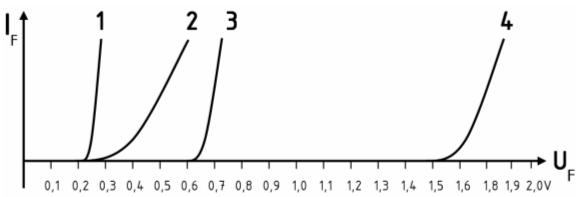
\includegraphics[scale=0.4]{Diode/Bilder/TC510a.png}
	\end{figure}

\mucho{7}{TC522}
{Welches sind die Haupteigenschaften einer Schottkydiode?}%Frage
{Sehr niedrige Durchlassspannung und sehr niedrige Schaltfrequenz.}%A
{Sehr niedrige Durchlassspannung und sehr hohe Schaltfrequenz.}%B
{Sehr hohe Durchlassspannung und sehr hohe Schaltfrequenz.}%C
{Sehr hohe Durchlassspannung und sehr niedrige Schaltfrequenz.}%D
{B}%Lösung


\aufgabentext{
	\begin{enumerate}
	\item[8] Das folgende Signal wird als U1 an den Eingang der Schaltung gelegt. Welches U2 ergibt sich bei Verwendung einer Silizum- und bei einer Germaniumdiode 
	\end{enumerate}
	\loesung{A Siliziumdiode; D Germaniumdiode}
	}

\begin{figure}[H]
	\centering
	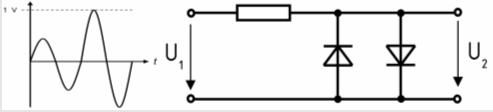
\includegraphics[scale=0.6]{Diode/Bilder/TC522.png}\\
	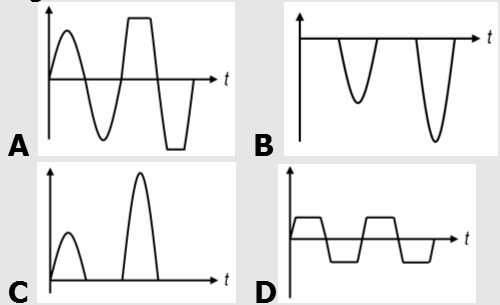
\includegraphics[scale=0.4]{Diode/Bilder/TC522ABCD.png}
	\end{figure}

\aufgabentext{
	\begin{enumerate}
	\item[9] Welche der folgenden Auswahlantworten enthält die richtige Diodenanordnung und Polarität eines Brückengleichrichters?
	\end{enumerate}
	A 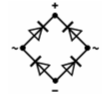
\includegraphics[scale=0.6]{Diode/Bilder/TD309A.png}
	B 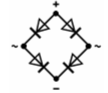
\includegraphics[scale=0.6]{Diode/Bilder/TD309B.png}
	C 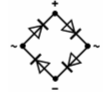
\includegraphics[scale=0.6]{Diode/Bilder/TD309C.png}
	D 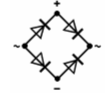
\includegraphics[scale=0.6]{Diode/Bilder/TD309D.png}
	\loesung{Lösung: A}
	}

	
